% arara: pdflatex
% arara: pdflatex
% arara: pdflatex

% options:
% thesis=B bachelor's thesis
% thesis=M master's thesis
% czech thesis in Czech language
% slovak thesis in Slovak language
% english thesis in English language
% hidelinks remove colour boxes around hyperlinks

\documentclass[thesis=B,czech]{FITthesis2}[2012/06/26]

\usepackage[utf8]{inputenc} % LaTeX source encoded as UTF-8

\usepackage{graphicx} %graphics files inclusion
% \usepackage{amsmath} %advanced maths
% \usepackage{amssymb} %additional math symbols

\usepackage{dirtree} %directory tree visualisation

\usepackage[shortlabels]{enumitem}

% % list of acronyms
% \usepackage[acronym,nonumberlist,toc,numberedsection=autolabel]{glossaries}
% \iflanguage{czech}{\renewcommand*{\acronymname}{Seznam pou{\v z}it{\' y}ch zkratek}}{}
% \makeglossaries

\newcommand{\tg}{\mathop{\mathrm{tg}}} %cesky tangens
\newcommand{\cotg}{\mathop{\mathrm{cotg}}} %cesky cotangens

% % % % % % % % % % % % % % % % % % % % % % % % % % % % % % 
% ODTUD DAL VSE ZMENTE
% % % % % % % % % % % % % % % % % % % % % % % % % % % % % % 

\department{Obor Webové a softwarové inženýrství (BI-WSI), zaměření Softwarové inženýrství\\Katedra softwarového inženýrství}
\title{Webová aplikace pro online web scraping}
\authorGN{Jakub} %(křestní) jméno (jména) autora
\authorFN{Drahoš} %příjmení autora
\authorWithDegrees{Jakub Drahoš} %jméno autora včetně současných akademických titulů
\author{Jakub Drahoš} %jméno autora bez akademických titulů
\supervisor{Martin Podloucký}
\keywordsCS{web scraping, extrakce dat, aplikace, JavaScript, rozšíření do Chromu}
\keywordsEN{web scraping, data extraction, application, JavaScript, Chrome extension}

\begin{document}
	
	% \newacronym{CVUT}{{\v C}VUT}{{\v C}esk{\' e} vysok{\' e} u{\v c}en{\' i} technick{\' e} v Praze}
	% \newacronym{FIT}{FIT}{Fakulta informa{\v c}n{\' i}ch technologi{\' i}}
	
	\begin{introduction}
		\paragraph*{Klíčová slova} \thekeywordscs{}
		\paragraph*{Keywords} \thekeywordsen{}
		
		\section*{Cíle práce}
		Hlavním cílem této práce je návrh a tvorba webové aplikace, která bude umožňovat uživatelům extrahovat požadovaná data z~libovolné stránky v~reálném čase bez jakékoli nutné znalosti programování. Při specifikaci požadavků tohoto softwaru se přihlídne k analýze stávajících řešení, jež je vedlejším cílem této práce. Druhým vedlejším cílem je poskytnout čtenáři úvod do právní problematiky web scrapingu a shrnout na jednom místě fakta, která máme k dispozici.
		
		Neméně důležitou součást práce tvoří dodržení klasického vývojového cyklu softwarového projektu -- analýza, design, implementace a testování.
		
		Klíčovým aspektem aplikace je též \emph{přehlednost a jednoduchost uživatelského rozhraní} -- důraz bude kladen na intuitivní a rychlé ovládání.
		
		Naopak v rozsahu této práce není tvorba web crawlera ani žádného jiného podobného mechanismu, jenž by systematicky a především \emph{automatizovaně} procházel danou oblast webu.
		
		\section*{Motivace}
		Téma web scrapingu je v dnešní době velice aktuální a čím více dat produkujeme, tím více bude stoupat potřeba tyto informace určitým způsobem získávat a zpracovávat. Téměř kdokoli, kdo pracuje s daty dostupnými z internetu, bude nucen využít nějaký nástroj k vytěžování, aby byl vůbec schopný udržet krok s konkurencí.
		
		Tedy důvod k vytvoření softwaru umožňující extrahovat data z webových stránek je jasný. Ač podobných nástrojů existuje několik, jejich obsluha je poměrně složitá a je nutné strávit určitý čas, než se člověk seznámí s jejich fungováním a může je naplno využít. Právě tento aspekt se snaží aplikace vyvíjená v rámci této bakalářské práce eliminovat -- motivací je tak poskytnout uživatelům možnost jednoduše a rychle vytěžit požadovaná data bez zbytečného zdržování a dlouhého času stráveného seznamováním se s nástrojem.
		
		Jak již bylo řečeno, přínos aplikace spočívá především v její jednoduchosti. Z toho mohou těžit uživatelé, kteří se nezabývají programováním nebo tvorbou webových stránek. Využije ji tak kdokoli, kdo potřebuje jednorázově získat data z libovolné internetové stránky, která obsahuje velké množství dat pohromadě na jedno místě. Z důvodu prozatím chybějícího crawlingu (automatizovaného procházení) je naopak nevhodná k pravidelnému získávání dat (jako je například dlouhodobé sledování cen produktů) či ke zpracování stránek, kdy se jednotlivá data nacházejí rozptýlená po celé doméně.
		
		\section*{Členění práce}
		Kapitola 1 je věnována analýze tématiky web scrapingu. První sekce shrnuje obecné informace, následuje pohled z právní strany věci a nakonec analýza stávajících řešení problému. Kapitola 2 se zaměřuje na návrh aplikace -- specifikace požadavků, architektura systému, návrh uživatelského rozhraní. Ve 3. kapitole je popsána realizace daného návrhu, výběr použitých technologií a odůvodnění rozhodnutí, která byla učiněna. Poslední kapitola je věnovaná testování celé aplikace.
	\end{introduction}
	
	
	% ================================================================================================
	
	
	\chapter{Analýza}
	
	\section{Analýza konkurenčních nástrojů}
	První skupinou, na kterou můžeme při hledání na internetu narazit, jsou společnosti, které nabízejí zákazníkům kompletní péči v~rámci extrakce dat. Cílí především na velké korporace, jimž postaví scrapovací nástroj přesně na míru, který poté také hostují a spravují. Zákazník tedy dostane data a o~nic víc se již nemusí starat. Jako příklad lze jmenovat třeba ContentGrabber, Mozenda a další.
	
	Pro tuto práci mnohem relevantnější kategorií je konkurenční nabídka nástrojů poskytujících uživatelům rozhraní k~web scrapingu. Zaměříme se pouze na takové nástroje, které nevyžadují jakoukoli znalost programování -- tedy žádné knihovny, API a nástroje pro budování vlastních scraperů.
	
	Mezi ty největší představitele patří ParseHub, Octoparse, WebScraper, Data Scraper a Dexi.io. Čtyři ze zmíněných nástrojů jsou volně dostupné (které mají však velmi omezenou funkcionalitu a pokročilejší operace se odemknou až s~určitým platebním plánem -- tzv. freemium model) a jeden poskytuje bezplatně pouze 7denní zkušební verzi.
	
	Předtím, než bude možné jednotlivé nástroje porovnávat, je nutné určit kritéria, podle kterých lze hodnotit kvalitu daného nástroje. Především půjde o~jednoduchost používání, celkovou přehlednost a rychlost, se kterou se uživatel dostane k~požadovaným datům. Důležitý je také způsob výběru dat, možnosti exportu získaných dat, jak aplikace sama dokáže uživatele seznámit s~používáním a také, v~jaké formě se nástroj vůbec používá a čím se od ostatních odlišuje (ať už v~pozitivním či negativním smyslu). 
	
	Poj\v{d}me se tedy na některé nástroje podívat blíže:
	
	\subsection{ParseHub}
	\textbf{Výhody:}
	\begin{itemize}
		\item výběr dat jak pomocí klikání (inteligentní hledání vzorců/podobností na základě prvních dvou kliknutí), tak pomocí XPath, regulárních výrazů nebo CSS selektorů
		\item aplikace obsahuje interaktivní tutoriál, který na jednoduchých příkladech ukáže, jak s~nástrojem zacházet
		\item možnost získání dat různými formami - přes API, jako CSV/XLS, do GoogleSheets nebo do Tableau
		\item různé módy kliknutí (výběr, relativní výběr, kliknutí), zooming in/out na HTML elementy -- když se uživatel netrefí (nebo ani trefit nemůže) přesně na požadovaný prvek, lze na něj lehce přejít pomocí této funkce
		\item automatická rotace IP adresy (tedy nedochází k~blokování ze strany serveru)
	\end{itemize}
	\textbf{Nevýhody:}
	\begin{itemize}
		\item nutnost stažení aplikace (ale je zde podpora pro Windows, Linux i Mac)
		\item aplikace je celkově těžkopádná, nemá moc přívětivé uživatelské rozhraní, ovládání působí nepřehledně a přehlceně -- na uživatele se vyvalí hodně informací a možností najednou
	\end{itemize}
	\begin{figure}[h]
		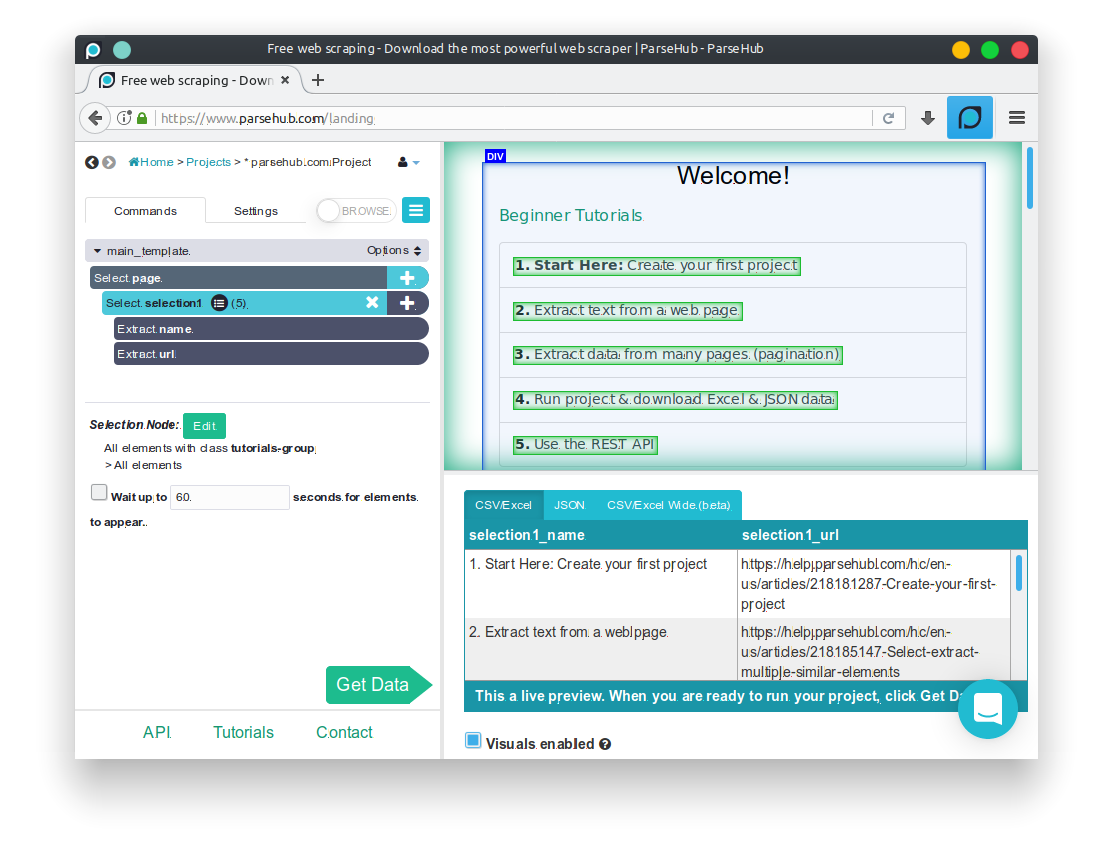
\includegraphics[width=\linewidth]{images/ParseHub.png}
		\caption{ParseHub\cite[snímek pořídil autor]{parsehub}}
		\label{fig:parseHub}
	\end{figure}
	
	
	\subsection{Octoparse}
	\textbf{Výhody:}
	\begin{itemize}
		\item výběr dat jak pomocí klikání (inteligentní hledání vzorců/podobností na základě prvních dvou kliknutí), tak pomocí XPath nebo regulárních výrazů
		\item nástroj obsahuje hotové šablony, které mohou velmi urychlit práci
		\item pestrá paleta možností (branch judgment, tvoření smyček apod.) -- dá se vytvořit téměř jakákoli logika procházení webu a extrakce dat
		\item lehký způsob, jak scrapování automatizovat
		\item možnost řídit tasky přes API (a získávat tak data taktéž přes API); data jdou nahrát rovnou i do lokální databáze
	\end{itemize}
	\textbf{Nevýhody:}
	\begin{itemize}
		\item nutnost stažení aplikace (která je navíc pouze pro Windows)
		\item těžkopádné a pomalé ovládání, neintuitivní rozhraní
		\item tutoriál je v~podstatě nic neříkající
		\item připravených šablon je jenom pár a jsou velmi konkrétní
	\end{itemize}
	\begin{figure}[h]
		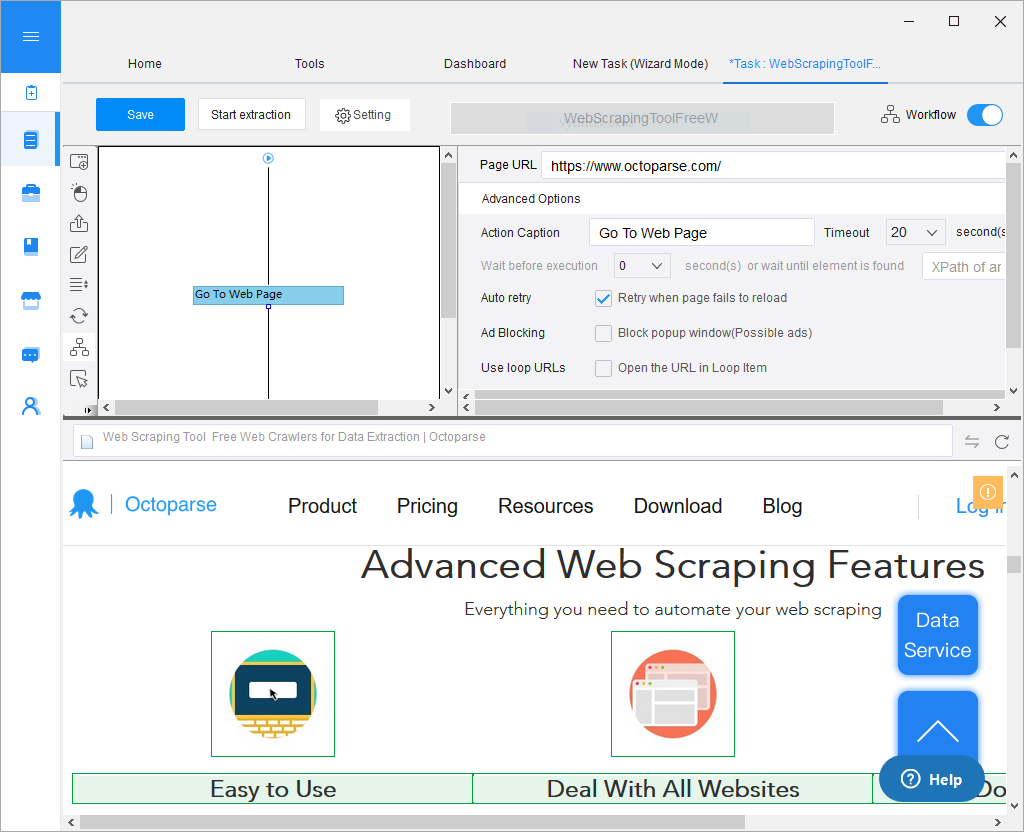
\includegraphics[width=\linewidth]{images/Octoparse.png}
		\caption{Octoparse\cite[snímek pořídil autor]{octoparse}}
		\label{fig:octoparse}
	\end{figure}
	
	
	\newpage
	\subsection{WebScaper}
	\begin{figure}
		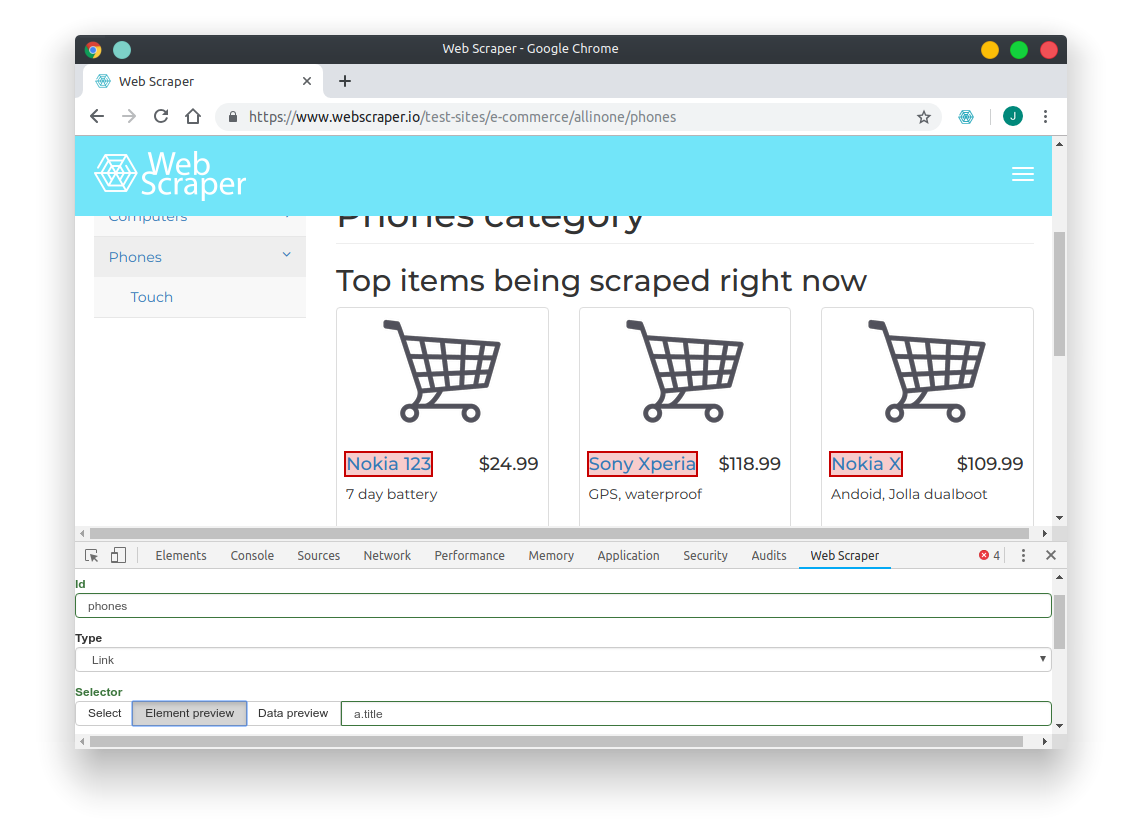
\includegraphics[width=\linewidth]{images/WebScraper.png}
		\caption{WebScraper\cite[snímek pořídil autor]{webscraper}}
		\label{fig:webScraper}
	\end{figure}
	\textbf{Výhody:}
	\begin{itemize}
		\item jednoduchá instalace (jedná se pouze o~rozšíření do prohlížeče Google Chrome); scrapování probíhá skrze vývojářskou konzoli
		\item výběr dat pomocí klikání (inteligentní hledání vzorců/podobností na základě prvních dvou kliknutí)
		\item tutoriály jsou formou videí -- jednoduché, rychlé a naprosto postačující
		\item různé typy elementů, které vybíráme (text, odkaz, scroll down), takže lze celkem snadno projít celou doménu
		\item možnost získání dat různými formami -- přes API, jako CSV/XLS nebo do Dropboxu
		\item klávesové zkratky při výběru elementů velmi usnadňují práci
		\item možnost využít jejich cloud k~automatizaci celého procesu
		\item oproti konkurenci nabízí přehledné rozhraní, rychlé a jednoduché používání
	\end{itemize}
	\textbf{Nevýhody:}
	\begin{itemize}
		\item nutnost používat Google Chrome, což pro některé uživatele může být překážka
		\item nelze vyhledávat podle klíčových slov ani podle HTML nebo CSS, tudíž všechno se musí manuálně naklikat
	\end{itemize}
	
	
	\subsection{Dexi.io}
	\begin{figure}[h]
		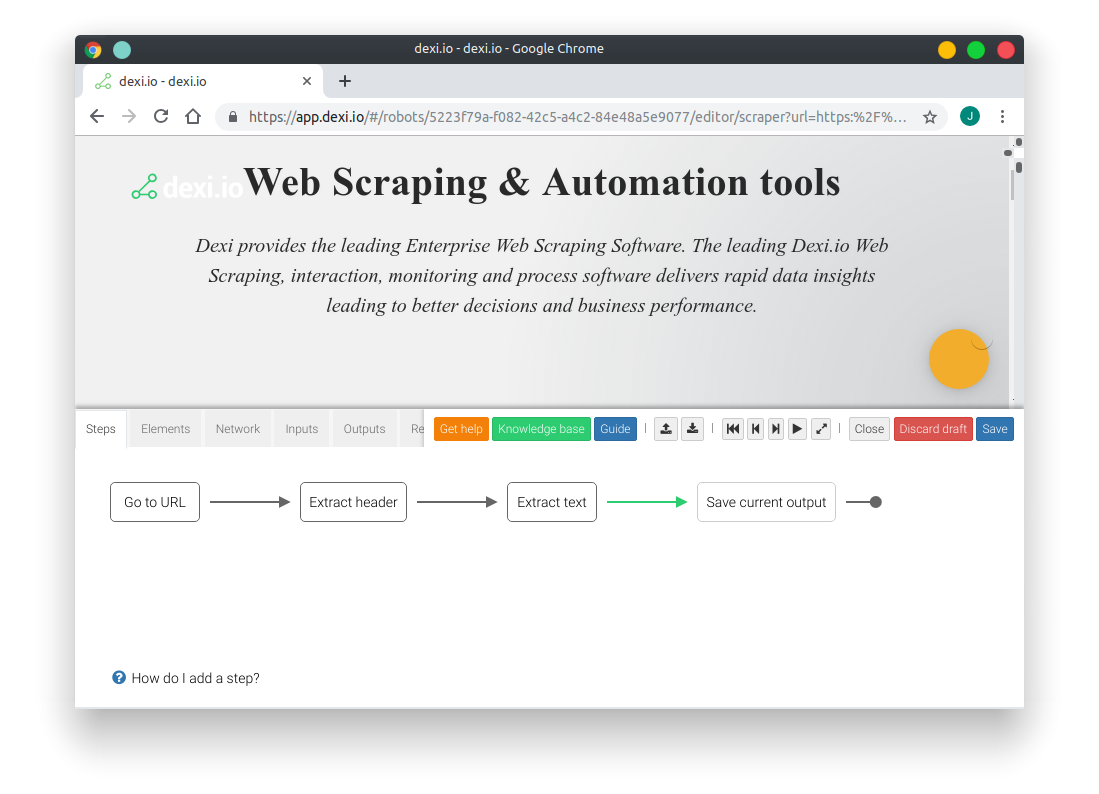
\includegraphics[width=\linewidth]{images/Dexiio.png}
		\caption{Dexi.io\cite[snímek pořídil autor]{dexio}}
		\label{fig:dexi.io}
	\end{figure}
	\textbf{Výhody:}
	\begin{itemize}
		\item bez nutnosti stahování aplikace -- vše se ovládá přes webové rozhraní
		\item výběr dat jak pomocí klikání (inteligentní hledání vzorců/podobností na základě prvních dvou kliknutí), tak pomocí HTML, CSS nebo textové shody
		\item mnoho návodů dostupných na stránkách, interaktivní rádce přímo při scrapování
		\item všechny možné druhy kliknutí, takže lze lehce projít celou doménu
		\item možnost exportovat data do CSV, JSON, XLS, získat přes API, poslat do Google Drive, Google Sheets nebo Amazon S3
		\item různé módy aplikace -- scraping, crawler, pipes (skládání menších scrape botů) a autobot (extrahování z~více stránek najednou se stejným rozložením); možnost takto automatizovat celý proces.
		\item nápomocné jsou různé addony (např. na obcházení Captchy)
	\end{itemize}
	\textbf{Nevýhody:}
	\begin{itemize}
		\item široká nabídka možností, a tak chvílí trvá, než se člověk zorientuje
		\item placený nástroj, zadarmo je dostupná pouze týdenní zkušební verze
		\item úvodní tutoriál je velmi strohý a žádné velké seznámení s~nástrojem se nekoná
	\end{itemize}
	
	
	\subsection{Data Scraper}
	\textbf{Výhody:}
	\begin{itemize}
		\item jednoduchá instalace (jedná se pouze o~rozšíření do prohlížeče Google Chrome).
		\item velmi jednoduché ovládání a přehledné rozhraní
		\item výběr dat probíhá pomocí klikání
		\item klikáním se utváří JQuery selektor, který si uživatel může podle svého upravit a doladit tak drobné detaily, jež by jinak nutně zahltily uživatelské rozhraní (tedy je možné vyhledávat i podle HTML tagů, id, CSS selektorů -- zkrátka vše, co umí klasické JQuery)
		\item různé druhy kliknutí
		\item možnost spustit na stránce libovolný JavaScriptový kód v~rámci scrapování
	\end{itemize}
	\textbf{Nevýhody:}
	\begin{itemize}
		\item nutnost používat Google Chrome, což pro některé uživatele může být překážka
		\item oproti ostatním nástrojům se může zdát velmi chudý na různé funkce
	\end{itemize}
	\begin{figure}
		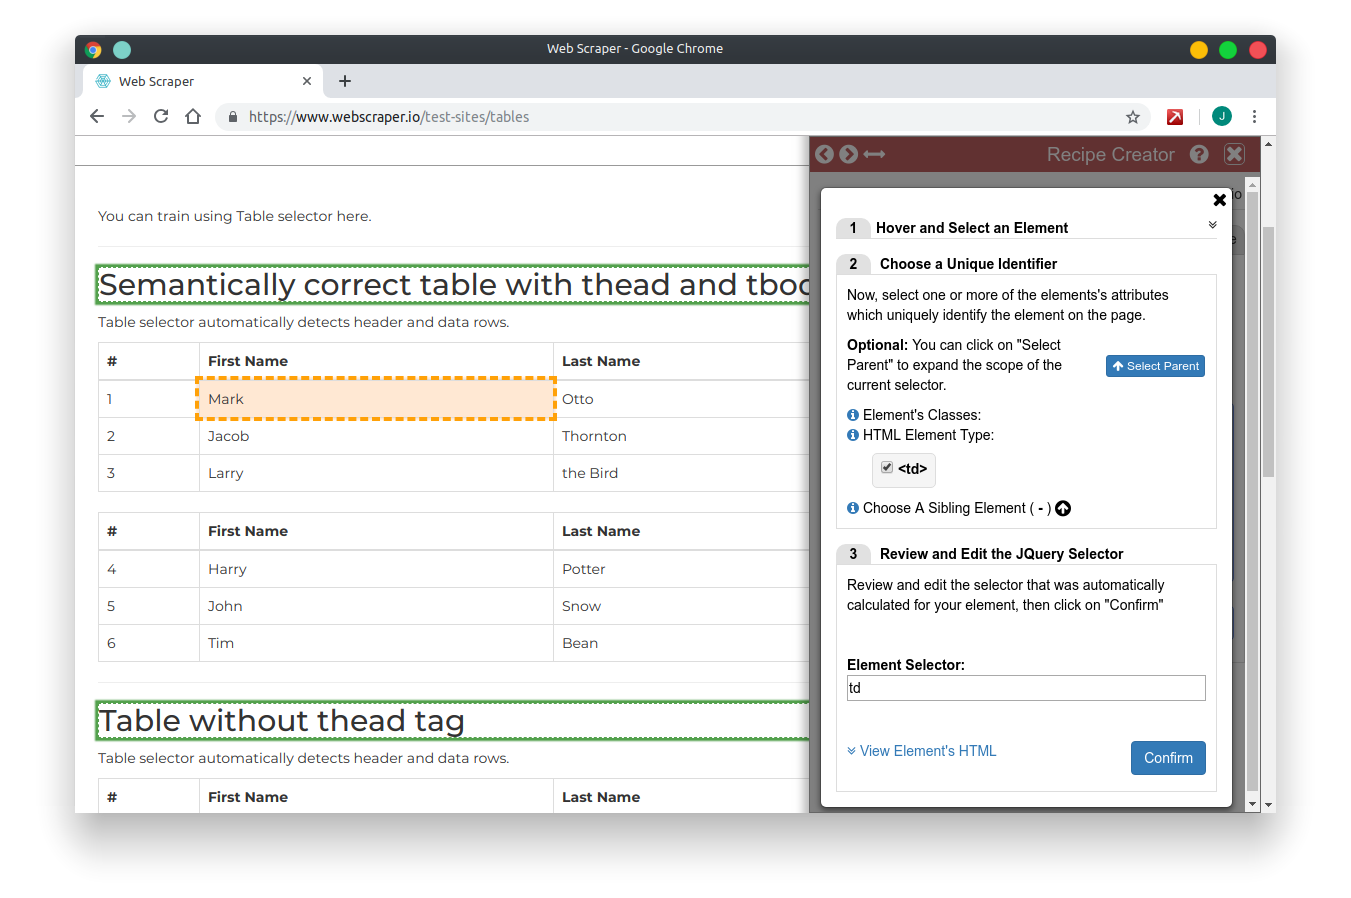
\includegraphics[width=\linewidth]{images/DataScraper.png}
		\caption{Data Scraper\cite[snímek pořídil autor]{data_scraper}}
		\label{fig:dataScraper}
	\end{figure}

	\subsection{Shrnutí}
	Jak jsme viděli, největšími neduhy, které se prolínají napříč valnou většinou aplikací, jsou \emph{těžkopádné uživatelské rozhraní}, \emph{neintuitivní ovládání} a \emph{rychlost} (nebo spíš pomalost), se kterou se uživatel dostane k~požadovaným datům. Také jsme se přesvědčili, že nejpříjemnější cestou je celou aplikaci ovládat přes webové rozhraní  \emph{bez nutnosti stahování a instalace}.
	
	Na druhou stranu se lze u~konkurence i inspirovat. Za vyzdvižení stojí určitě \emph{různé druhy výběru dat} -- \emph{klikání} přímo na stránce spolu s~inteligentním hledáním podobných prvků jistě tvoří mocný mechanismus. Avšak je potřeba zajistit i ostatní způsoby výběru (jako je např. \emph{textová shoda, HTML tagy, CSS selektory}) pro případ, kdy je pouhé klikání zdlouhavé či nevyhovující. Rovněž široký výběr způsobů exportu dat, intuitivní klávesové zkratky a zooming in/out na prvky může uživatelům zpříjemnit práci s~nástrojem.
	
	% ================================================================================================
	
	\chapter{Realizace}
	
	\section{Zvolené řešení}
	
	
	% ================================================================================================
	
	
	\begin{conclusion}
		%sem napište závěr Vaší práce
	\end{conclusion}
	
	\bibliographystyle{csn690}
	
	\begin{thebibliography}{9}
		\bibitem{parsehub}
		PARSEHUB. \textit{ParseHub. Version 54.0.1} [software]. 2015 [cit. 13. 4. 2019]. Dostupné z: \url{https://www.parsehub.com/quickstart}.
		
		\bibitem{octoparse}
		OCTOPUS DATA INC. \textit{Octoparse. Version 7.1.2} [software]. 2018 [cit. 13. 4. 2019]. Dostupné z: \url{https://www.octoparse.com/download}.
		
		\bibitem{webscraper}
		WEBSCRAPER. \textit{WebScraper. Version 0.3.8.9} [software]. 2016 [cit. 13. 4. 2019]. Dostupné z: \url{https://chrome.google.com/webstore/detail/web-scraper/jnhgnonknehpejjnehehllkliplmbmhn}.
		
		\bibitem{dexio}
		DEXI APS. \textit{Dexi.io} [software] [cit. 13. 4. 2019]. Dostupné z: \url{https://app.dexi.io/}.
		
		\bibitem{data_scraper}
		SOFTWARE INNOVATION LAB LLC. \textit{Data scraper. Version 3.299.84} [software]. 2015 [cit. 13. 4. 2019]. Dostupné z: \url{https://chrome.google.com/webstore/detail/data-scraper-easy-web-scr/nndknepjnldbdbepjfgmncbggmopgden}.
		
	\end{thebibliography}

	\appendix
	
\end{document}
